In questo capitolo presenterò la logica della \textit{versione base} del protocollo GreenWUP così come è descritto e presentato in letteratura. Presenterò inoltre una procedura chiamata \textit{Interest Dissemination}, usata per inizializzare informazioni come l'\textit{hop count} di ogni nodo della rete.  

\section{Interest Dissemination (FloodWUP)}
La fase di \textit{Interest Dissemination} è una procedura molto importante per il corretto funzionamento di GreenWUP. In particolare questa fase viene realizzata attraverso un protocollo di \textit{flooding} chiamato FloodWUP, descritto in \cite{greenWup}. \\

L'obbiettivo principale di questo protocollo è far si che ogni nodo della rete riesca a impostare la propria distanza dal sink (espressa in numeri di hop, ovviamente).\\
Da qui in avanti si farà riferimento a questo valore mediante il termine \textit{hopCount}.\\ 

La procedura ha inizio con l'invio di una pacchetto chiamato \textit{disseminationPacket} (per semplicità DP) da parte del sink. Questo pacchetto conterrà il valore che i vari nodi useranno come proprio hopCount. In particolare questo valore vale 0 solo per il sink, mentre ogni nodo che riceve il pacchetto memorizza il proprio valore come \( valore\_pacchetto + 1 \). \\

Una particolarità molto importante di questo protocollo è che il traffico generato, seppur l'invio segua un process di broadcast, non genera \textit{broadcast storm}. Ciò è ovviamente possibile grazie all'uso dei messaggi di wake-up e grazie al fatto che ogni nodo usa un pool condiviso di indirizzi di wake-up \(w_1, w_2....w_n\).\\
Inizialmente i vari nodi usano l'indirizzo \(w_1\) per cui il sink, così come gli altri nodi, durante l'invio del primo DP sveglierà i propri vicini usando l'indirizzo \(w_1\). Ogni nodo, dopo aver ricevuto il DP, procede a cambiare indirizzo di wake-up da \(w_1\) a \(w_2\) e a ridistribuire il DP corrente ai suoi vicini usando però l'indirizzo con cui sono stati svegliati (nel caso del primo pacchetto DP \(w_1\)).\\

Con l'invio del secondo DP, invece, i vari nodi useranno allo stesso modo \(w_2\), così come per il terzo DP useranno \(w_3\) e così via. Questo permette di evitare il \textit{broadcast storm} in quanto i nodi che hanno già ricevuto un pacchetto DP, avendo aggiornato la sequenza di wake-up, non riceveranno duplicati di questo.

\begin{listing}[h]
    \caption{Procedura usata dal Sink per creare un nuovo DisseminationPacket}
    \label{code:createDP}
    \begin{minted}[mathescape, linenos, numbersep=10pt, gobble=0, fontsize=\small, frame=lines, framesep=2mm]{cpp}

GreenWupPacket* macFrame;
macFrame = new GreenWupInterest("GreenWupInterest", MAC_LAYER_PACKET);

// Informazioni per DisseminationPacket
macFrame->setWurAddress(wurDisseminationAddresses[fromNetAddressIndex]);
macFrame->setType( PKT_GREEN_WUP_INTEREST );
macFrame->setHc(level);
int size = wurDisseminationAddresses.size();
fromNetAddressIndex = ( fromNetAddressIndex + 1 ) % ( size );

// Informazioni Generiche
encapsulatePacket(macFrame, pkt);
macFrame->setDestination(destination);
macFrame->setNetAddress(self);
macFrame->setNetSN(netSN++);
macFrame->setSource(SELF_MAC_ADDRESS);

    \end{minted}
\end{listing} \\

Come mostrato nel \textbf{Codice \ref{code:createDP}}, il nodo sink imposta alcuni parametri come \textit{sequenza di wake-up}, il \textit{tipo del pacchetto} (usato dai vicini che ricevono il pacchetto in modo da gestirlo nel corretto modo) e ovviamente l' \textit{hopCount}. Fatto ciò aggiorna il prossimo indirizzo di wake-up da usare (\textbf{linea 9, Codice \ref{code:createDP}}) e invia il pacchetto in broadcast. \\

Ciò che invece mostra il \textbf{Codice \ref{code:forwardDP}} è il modo in cui i vari nodi gestiscono il \textit{DisseminationPacket} una volta ricevuto. Come si può notare la prima cosa che fanno è aggiornare il proprio \textit{hopCount} e successivamente, se il pacchetto non è un duplicato, procedono con l'aggiornare il valore contenuto nel pacchetto e all'invio di questo in broadcast.\\
Ovviamente aggiornano, proprio come il sink, la sequenza di wake-up valida per ricevere il prossimo \textit{DisseminationPacket}. \\
\'E interessante notare la presenza del controllo a \textbf{riga 5 ,Codice \ref{code:forwardDP}}: nonostante  il protocollo dovrebbe evitare la ricezione di duplicati automaticamente, questo fenomeno potrebbe comunque accadere. Infatti, potrebbe capitare che un vicino attivo (in modalità RX), che sta facendo attività come CARRIER SENSING, riceva un \textit{DisseminationPacket} duplicato. Grazie a questo controllo si eviterebbe la ritrasmissione di un pacchetto duplicato.

\begin{listing}[h]
    \caption{Procedura usata dai nodi per la gestione del DisseminationPacket}
    \label{code:forwardDP}
    \begin{minted}[mathescape, linenos, numbersep=10pt, gobble=0, fontsize=\small, frame=lines, framesep=2mm]{cpp}

GreenWupInterest *macPkt = dynamic_cast <GreenWupInterest*>(pkt);

updateLevel ( macPkt->getHc() );

if ( isNotDuplicatePacket(pkt) == false ){
  collectOutput("MAC", "Duplicated packets");
  return;
}

GreenWupInterest *newPkt = dynamic_cast <GreenWupInterest*>(pkt->dup());
newPkt->setHc(level);

wurModule->removeWakeupAddress( wurDisseminationAddresses[addressIndex] );

int size = wurDisseminationAddresses.size();
addressIndex = ( addressIndex + 1 ) % ( size );
wurModule->addWakeupAddress( wurDisseminationAddresses[addressIndex] );

    \end{minted}
\end{listing} \\

Ovviamente durante l'intera procedura di \textit{Interest Dissemination} si prevede l'invio di \(n\geq1\) \textit{DisseminationPacket} in modo da essere sicuri che tutti i nodi della rete siano in grado di stabilire la propria distanza dal centro.\\
Ogni pacchetto viene inviato dopo un intervallo di tempo rispetto al precedente abbastanza grande da permettere il termine della precedente fase di Interest Dissemination. \\
Per la realizzazione di questo progetto sono stati previsti 3 ripetizioni della procedura di \textit{Interest Dissemination} in modo da essere sicuri che tutti i nodi della rete abbiano impostato il loro hopCount.

\newpage

\begin{figure}[t!]
  \begin{subfigure}[t]{.8\linewidth}
    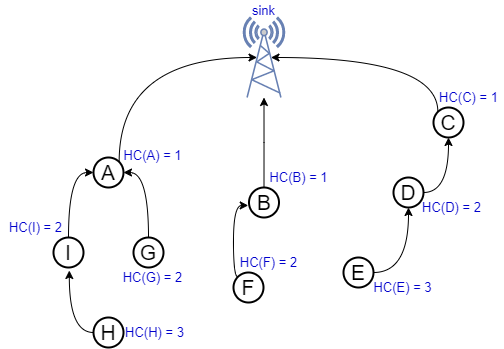
\includegraphics[width=1.1\linewidth]{Contents/Images/graphs/interestDissemination/hopCount.png}
  \end{subfigure}
  \caption{Stato della rete una volta finita la fase di Interes Dissemination}
  \label{fig:hopCount}
\end{figure}

Una volta terminata interamente la fase di \textit{Interest Dissemination}, lo stato della rete è quello mostrato in  \textbf{Figura \ref{fig:hopCount}} dove ogni nodo è a conoscenza della distanza tra se stesso e il sink. 

\section{Il protocollo GreenWUP}
GreenWUP, presentato in \cite{greenWup}, è un protocollo \textit{cross-layer} (Routing + MAC) usato nelle \textit{Green Wireless Sensor Network} che fa uso di tecnologie come \textit{energy-harvesting}, \textit{wake-up radio} e \textit{semantic-addressing} al fine di migliorare il consumo energetico della rete e in generale le sue prestazioni.  \\

GreenWUP è un protocollo \textit{converge-casting} basato sugli \textit{hop-count}. Infatti, è molto importante che ogni nodo della rete sia a conoscenza della propria distanza dal sink in termini di hop.\\
Questo valore, nel caso di GreenWUP, è calcolato automaticamente, infatti, conoscendo il raggio di azione delle 2 antenne (principale e di wake-up) e conoscendo la posizione esatta dei nodi è possibile stabilire per ogni nodo la sua distanza dal sink.\\

Tuttavia per questo progetto si è deciso di calcolare questo valore mediante un prima fase iniziale chiamata \textit{Interest Dissemination} usando il protocollo \textit{FloodWUP}.\\

Altra caratteristica molto importante per il corretto funzionamento di GreenWUP è che ogni nodo ha associato, all'interno di una stessa rete, due indirizzi di wake-up:
\begin{enumerate}
    \item \textbf{w\textsubscript{ID}}, un indirizzo statico che identifica univocamente il nodo all'interno della rete 
    \item \textbf{w\textsubscript{LE}}, un indirizzo dinamico con semantica che identifica lo stato in cui un nodo si trova in un determinato istante
\end{enumerate}
L'indirizzo \textbf{w\textsubscript{ID}} è un semplice intero progressivo che identifica i vari nodi assegnando un ID da \textit{0} a \textit{n} se si hanno \textit{n} nodi.\\
L'indirizzo \textbf{w\textsubscript{LE}}, invece, è ricalcolato periodicamente in quanto deve rappresentare lo stato attuale del nodo. In particolare è formato da due sequenze \(w_{L}w_{E}\) dove w\textsubscript{L} è la codifica del valore di hop-count del nodo e w\textsubscript{E} è l'energia residua del nodo. Nello specifico i vari livelli di energia sono discretizzati in \textit{k} classi\footnote{Ogni classe comprende un range di valori di energia, per cui un nodo con energia residua \textit{x} appartiene alla classe \textit{k} sse \(energiaResidua(nodo)\in range(\texitf{k})\)} per cui w\textsubscript{E} è la classe energetica a cui, attualmente, il nodo appartiene.\\

\'E possibile dividere in fasi l'invio di un  pacchetto DATA, inviato ovviamente da un nodo \textit{sender}\footnote{Nodo che detiene un pacchetto DATA da inoltrare verso il \textit{sink}} verso il \textit{next-hop}\footnote{Nodo vicino al \textit{sender} che riceve il pacchetto DATA da questo}:
\begin{itemize}
    \item \textit{Relay Selection}: in questa prima fase il sender prova ad instaurare una comunicazione con i receiver\footnote{Nodi vicini del sink che potrebbero essere scelti come \texitit{next-hop} }. Infatti si utilizza l'indirizzo di wake-up \textbf{w\textsubscript{LE}}. Questa procedura si considera conclusa nel momento in cui il nodo sender ha scelto, tra i propri vicini, chi sarà il next-hop.
    \item \textit{Send DATA}: in questa fase il nodo sender sollecita, mediante l'indirizzo di wake-up \textbf{w\textsubscript{ID}}, il next-hop e procede poi con l'invio del pacchetto DATA.
    \item \textit{Send ACK}: in questa fase finale il nodo next-hop, dopo aver correttamente ricevuto il pacchetto DATA, invia un ACK al nodo sender in modo da confermare la ricezione.
\end{itemize}
Un'osservazione importante è che se il next-hop si trova a distanza 1 dal sink, la fase di \textit{Relay Selection} viene saltata. Infatti il nodo sink è sempre in ascolto per cui si procede direttamente con l'invio del pacchetto DATA e con il successivo pacchetto ACK.\\\\

\begin{figure}[h!]
  \begin{subfigure}[t]{.8\linewidth}
    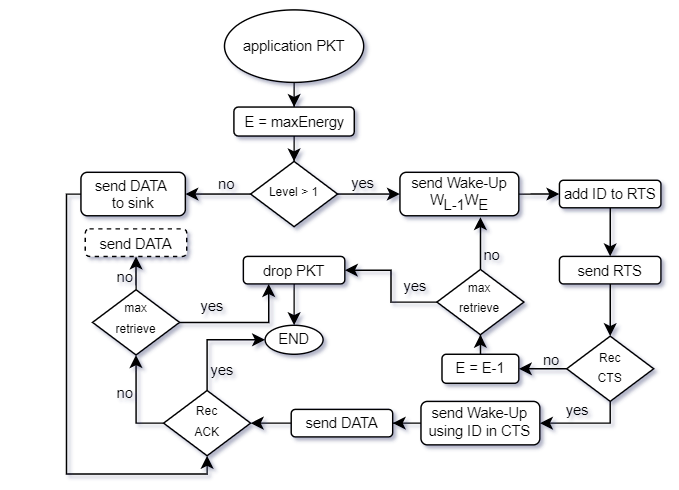
\includegraphics[width=1.15\linewidth]{Contents/Images/schemes/greenWupBase/GreenWup_base_sender.png}
  \end{subfigure}
  \caption{Logica funzionamento nodo \texitit{sender}}
  \label{fig:logicaSender}
\end{figure}

La \textbf{Figura \ref{fig:logicaSender}} sopra riportata mostra il comportamento di un nodo sender una volta che questo ha un pacchetto DATA da gestire.\\

Bisogna precisare che il nodo sink si occuperà della sola ricezione di pacchetti DATA per cui mai per nessun motivo il sink eseguirà questa procedura.\\
Come mostrato dalla \textbf{Figura \ref{fig:logicaSender}}, all'inzio la classe di energia considerata è la massima. A questo punto se il nodo è un vicino del sink, per cui \(level=1\), si salta come già detto la fase di Relay Selection e si invia direttamente il dato al sink. Altrimenti vengono sollecitati i vicini in base alla loro distanza dal sink e alla loro classe energetica. Si noti che il sender memorizza all'interno del pacchetto RTS il proprio indirizzo univoco in modo da essere ricontattato poi per ricevere il CTS.\\
Qualora non dovesse ricevere nessun pacchetto CTS, il sender riproverebbe con una classe energetica più bassa un numero massimo di volte, per poi eliminare il pacchetto e terminare la procedura.\\
Se, invece, il nodo sender dovesse ricevere il pacchetto CTS, solleciterebbe il vicino usando l'indirizzo univoco contenuto all'interno del CTS per poi mandaere il pacchetto DATA e successivamente si metterebbe in attesa dell'acknowledge. Se il nodo riceve l'ACK allora conclude la procedura, altrimenti ritenta l'invio del pacchetto per un massimo numero di volte per poi eliminarlo e terminare la procedura.\\\\

\begin{figure}[h!]
  \begin{subfigure}[t]{.8\linewidth}
    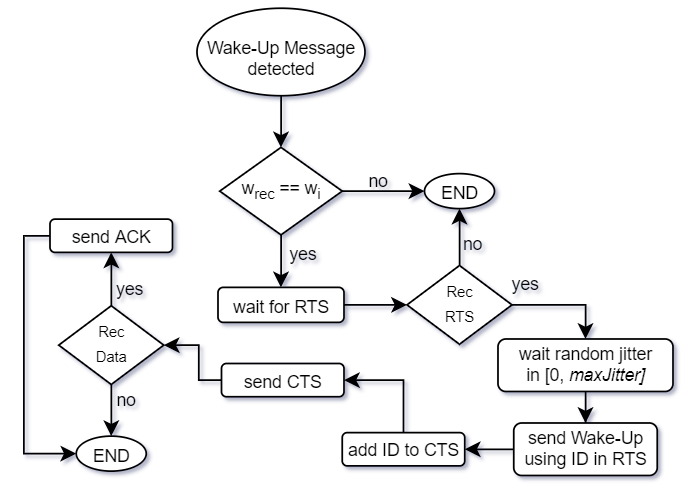
\includegraphics[width=1.1\linewidth]{Contents/Images/schemes/greenWupBase/GreenWup_base_receiver.png}
  \end{subfigure}
  \caption{Logica funzionamento nodo \texitit{receiver}}
  \label{fig:logicaReceiver}
\end{figure}

La \textbf{Figura \ref{fig:logicaReceiver}} sopra riportata mostra il comportamento di un nodo receiver una volta che questo viene sollecitato da un vicino tramite un messaggio di wake-up.\\
La prima cosa che fa un nodo receiver è controllare che la sequenza di wake-up con cui è stato sollecitato corrisponda a \(w_{i}\) dove \(w_{i} \in (w_{ID}, w_{LE})\). Se così non dovesse essere allora ignora il pacchetto e la procedura finisce, altrimenti si mette in attesa di un pacchetto RTS da parte del sender. Una volta ricevuto si aspetta un tempo calcolato randomicamente per poi sollecitare il nodo sender usando le informazioni contenute nel pacchetto RTS. Una volta sollecitato il nodo sender, il receiver procede con la creazione del pacchetto CTS con le proprie informazioni e, una volta creato, lo invia al sender.\\
A questo punto il receiver non può far altro che mettersi in attesa del pacchetto DATA. Ovviamente solo il receiver scelto come \textit{next-hop} riceverà il pacchetto DATA, per poi proseguire con l'invio dell'acknowledge. Per tutti gli altri scatterà un \textit{timeout} che terminerà la procedura.

\newpage

\section{Problematiche GreenWUP}
In questo paragrafo descriverò problematiche derivanti da mie osservazioni o da determinati risultati ottenuti durante il testing della versione base del protocollo.\\

Una prima osservazione ricade sulla fase di Relay-Selection e quindi sullo scambio dei pacchetti RTS/CTS con i wake-up message e tempi che ne derivano. GreenWUP, infatti, prevede che ad ogni nuovo pacchetto data, il nodo sender debba scegliere tra i propri vicini il next-hop che si occuperà di inoltrare il pacchetto verso il sink. Ovviamente questa è la procedura che più richiede tempo e spreco di energia per cui ripeterla sempre potrebbe essere inefficace soprattutto in scenari con traffico denso. Potrebbe, quindi, avere senso tenere traccia in qualche modo delle varie scelte che i nodi sender fanno durante l'intera simulazione in modo da ridurre il numero di ripetizioni di questa procedura.\\

Una seconda osservazione, strettamente collegata alla prima, ricade sul fatto che dall'altra parte i nodi receiver, una volta ricevuta una stringa di wake-up, non hanno nessuna logica decisionale riguardo l'attivarsi o meno in ascolto, infatti, da protocollo attivano la main radio in RX.\\
Ovviamente ciò comporta che in fase di Relay-Selection, ad esempio, tutti i receiver partecipano alla fase e, dato che solo uno poi sarà scelto come next-hop, tutti gli altri nodi non faranno altro che sprecare energia inutilmente. Se invece potessero decidere di non partecipare alla fase, evitando quindi di settare la radio principale a RX, potrebbero risparmiare energia. Ovviamente questo è un aspetto abbastanza complesso su cui bisogna prestare attenzione nello scegliere le condizioni con il quale un nodo decide o meno di attivarsi in RX o meno, in quanto potrebbe capitare che nessun nodo decida di partecipare alla fase di Relay-Selection rischiando non solo ripetizioni della fase, ma anche la perdita del pacchetto se dovesse essere raggiunto il limite di tentativi.\\

Infine, studiando l'implementazione della versione base del protocollo si può notare come ogni nodo receiver aspetti un Jitter puramente randomico prima di inviare il pacchetto CTS al sender. Potrebbe risultare utile sfruttare al meglio questo valore calcolandolo non randomicamente ma in funzione dell'energia residua, come succede in \textbf{GreenRoutes}\cite{greenRoutes}. In questo modo il nodo sender riceverebbe il pacchetto CTS dal nodo con più energia e, dato che viene scelto il primo CTS ricevuto, si eviterebbe di scegliere come next-hop un nodo al limite della classe energetica corrente.